%=====================================================================
% EAIFR THESIS TEMPLATE — VERSION 3 (RICH, BROCHURE-STYLE COVER)
% East African Institute for Fundamental Research
%
% Style : tasteful navy + gold palette drawn from the EAIFR brochure.
%         Cover page with a subtle black-and-white Virunga mountain
%         silhouette behind a serif title, first letters highlighted
%         in gold (E A I F R), a thin gold rule and an italic tagline.
%         Inside: simple gold-underlined chapter headings. EAIFR only
%         — no partner institution logos.
%=====================================================================

% openany : do not force chapters to start on a recto page, so we
%           don't get spurious blank verso pages between short chapters.
\documentclass[12pt, a4paper, openany]{book}

% ---------- Typography & layout ----------
\usepackage[protrusion=true,expansion=true]{microtype}
\usepackage[utf8]{inputenc}
\usepackage[english]{babel}
% For Greek in text mode, uncomment: \usepackage[greek,english]{babel}\usepackage{alphabeta}
\usepackage[margin=1in,headheight=15pt]{geometry}
\setlength{\parskip}{2mm}
\setlength{\parindent}{1cm}

% ---------- Math ----------
\usepackage{amssymb,amsmath,bm,mathalfa}
% \usepackage{commath}  % Overleaf has it; remove this line if your TeX install lacks it

% ---------- xcolor MUST come before tikz to avoid option clash ----------
\usepackage[table]{xcolor}

% ---------- Graphics & floats ----------
\usepackage{graphicx}
\graphicspath{{figures/}}
\usepackage{wrapfig}
\usepackage{booktabs}
\usepackage{multirow}
\usepackage{array}
\usepackage{tabularx}
\usepackage{subcaption}
\usepackage{rotating}
\usepackage{adjustbox}
\usepackage{pdflscape}
\usepackage{lscape}
\usepackage{tikz}
\usetikzlibrary{calc,fadings}

% ---------- Misc ----------
\usepackage{verbatim}
\usepackage{spverbatim}
\usepackage{natbib}
\usepackage{appendix}
\usepackage{lipsum}

% ===================== EAIFR BRAND PALETTE ===========================
% Colours sampled from the official EAIFR brochure cover.
\definecolor{eaifrNavy}{HTML}{0F2A4A}    % deep institutional navy
\definecolor{eaifrNavyDark}{HTML}{0A1E36} % slightly deeper for gradients
\definecolor{eaifrGold}{HTML}{D4A04B}    % warm amber accent
\definecolor{eaifrCream}{HTML}{F5F1E8}   % warm off-white
\definecolor{eaifrGrey}{HTML}{5A5A5A}

% ---------- Links ----------
\usepackage[hidelinks]{hyperref}
\hypersetup{
  colorlinks=true,
  linkcolor=eaifrNavy,
  citecolor=eaifrNavy,
  urlcolor=eaifrGold,
}

% ---------- Running headers ----------
\usepackage{fancyhdr}
\pagestyle{fancy}
\fancyhf{}
\fancyhead[LE]{\small\color{eaifrNavy}\itshape\leftmark}
\fancyhead[RO]{\small\color{eaifrNavy}\itshape\rightmark}
\fancyhead[LO,RE]{\small\color{eaifrGrey}\scshape EAIFR}
\fancyfoot[C]{\small\color{eaifrGrey}\thepage}
\renewcommand{\headrulewidth}{0.3pt}
\renewcommand{\footrulewidth}{0pt}

% ---------- Chapter & section styling ----------
% Tasteful: chapter name and number on one line, gold rule beneath.
\usepackage{titlesec}
\titleformat{\chapter}[hang]
  {\normalfont\LARGE\bfseries\color{eaifrNavy}}
  {\color{eaifrGold}\chaptertitlename\ \thechapter\ \ \textbar\ \ }{0pt}
  {\LARGE}
  [\vspace{4pt}{\color{eaifrGold}\titlerule[1pt]}\vspace{4pt}]
\titlespacing*{\chapter}{0pt}{-20pt}{20pt}

\titleformat{\section}
  {\normalfont\Large\bfseries\color{eaifrNavy}}{\thesection}{1em}{}
\titleformat{\subsection}
  {\normalfont\large\bfseries\color{eaifrNavy!85!black}}{\thesubsection}{1em}{}

% TOC styling — a hint of gold
\usepackage{tocloft}
\renewcommand{\cftchapfont}{\bfseries\color{eaifrNavy}}
\renewcommand{\cftchappagefont}{\color{eaifrNavy}}
\renewcommand{\cftsecfont}{\color{black!80}}

\newcolumntype{L}{>{\centering\arraybackslash}m{3cm}}

% ---------- Document metadata (edit these) ----------
\newcommand{\thesistitle}{The Title of Your Thesis}
\newcommand{\thesissubtitle}{An optional subtitle}
\newcommand{\thesisauthor}{Author Name}
\newcommand{\thesisdegree}{Master of Science in Physics}
\newcommand{\thesissupervisor}{Prof.\ Supervisor Name}
\newcommand{\thesiscosupervisor}{Dr.\ Co-supervisor Name}
\newcommand{\thesisyear}{\the\year}
\newcommand{\thesislocation}{Kigali, Rwanda}

%=====================================================================

% Override \mainmatter so it does \clearpage (not \cleardoublepage),
% preventing a forced blank verso between the front- and main-matter.
\makeatletter
\renewcommand\mainmatter{\clearpage\@mainmattertrue\pagenumbering{arabic}}
\renewcommand\backmatter{\clearpage\@mainmatterfalse}
\makeatother

\begin{document}
\frontmatter

% =====================================================================
% COVER PAGE
% Full-bleed navy backdrop with a subtle Virunga cone silhouette behind
% the title. Serif "E A I F R" treatment with gold capitals, echoing
% the official EAIFR brochure.
% =====================================================================
\begin{titlepage}
\thispagestyle{empty}
\newgeometry{margin=0pt}

% ----- Background: navy base + mountain + navy veil (no hard bands) -----
% The mountain is pre-cropped to A4 aspect with the peak at ~55% vertical,
% so the wordmark can sit in the sky above the peak and the title block in
% the foothills below, both anchored at fixed fractions of the page.
\begin{tikzpicture}[remember picture, overlay]
  \fill[eaifrNavy] (current page.north west) rectangle (current page.south east);
  \node[opacity=1.0, inner sep=0pt, anchor=center] at (current page.center)
    {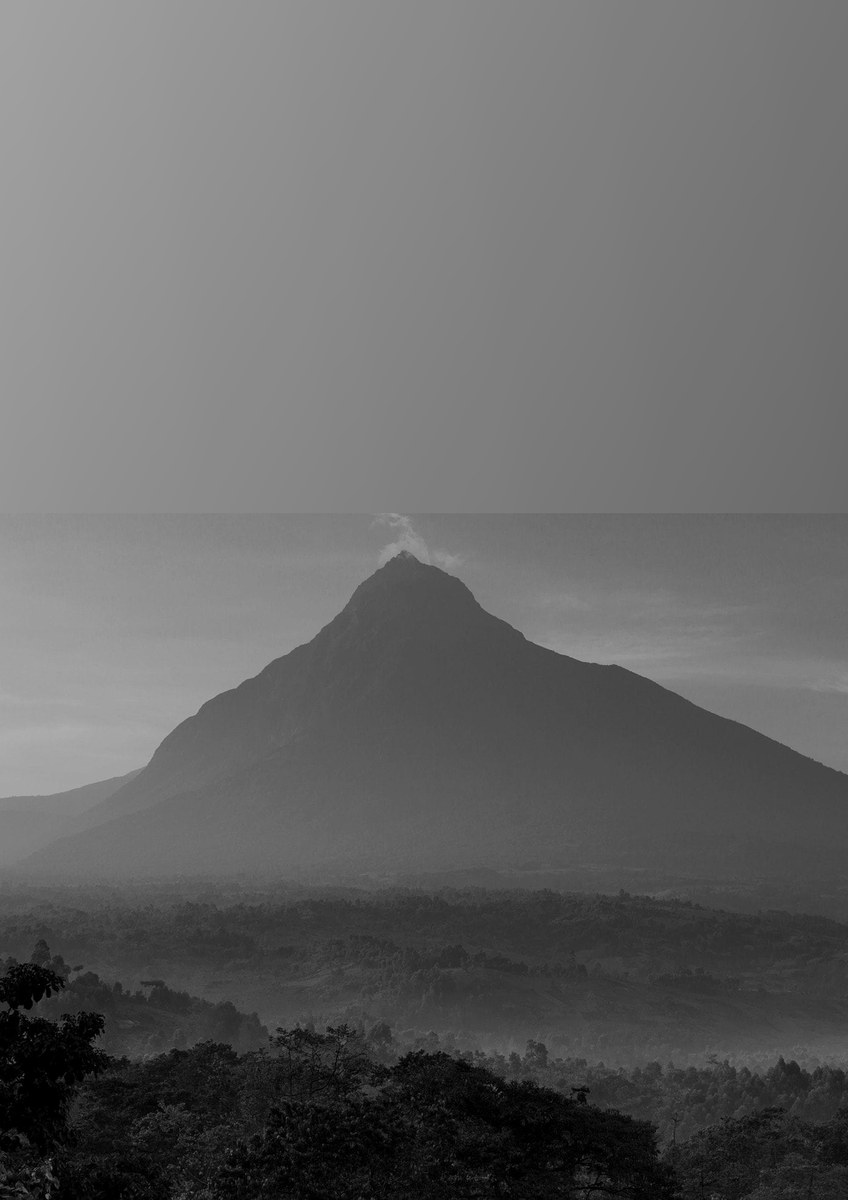
\includegraphics[width=\paperwidth]{virunga.jpg}};
  % Light navy veil — preserves the mountain silhouette while keeping brand.
  \fill[eaifrNavy, opacity=0.35]
    (current page.north west) rectangle (current page.south east);
  % Soft top vignette (stacked thin bands — no hard edge) for header legibility.
  \foreach \i in {1,...,5}{%
    \fill[eaifrNavyDark, opacity=0.07]
      (current page.north west) rectangle
      ($(current page.north east)+(0,-\i*0.8cm)$);
  }
  % Soft bottom vignette for the title block.
  \foreach \i in {1,...,6}{%
    \fill[eaifrNavyDark, opacity=0.08]
      ($(current page.south west)+(0,\i*1.2cm)$) rectangle
      (current page.south east);
  }
\end{tikzpicture}

% ----- Foreground text blocks at fixed page fractions -----
% Page fractions (measured from top):
%   0.07  — institute header band
%   0.28  — wordmark block centre (sits in the sky)
%   0.47  — tagline (just above the peak)
%   0.80  — title + author block centre (foothills area)
\begin{tikzpicture}[remember picture, overlay,
                   every node/.style={text=eaifrCream, align=center}]

  % --- Institute header (7% from top) ---
  \node[anchor=north, yshift=-1.7cm] at (current page.north)
    {\begin{minipage}{0.84\paperwidth}\raggedright
       {\small\scshape\sffamily East African Institute for Fundamental Research}%
       \hfill
       {\small\sffamily\color{eaifrGold}\thesisyear}\\[4pt]
       \textcolor{eaifrGold}{\rule{\linewidth}{0.6pt}}
     \end{minipage}};

  % --- Stacked EAIFR wordmark, centred at 25% of page height ---
  \node[anchor=center] at ($(current page.north)+(0,-0.25\paperheight)$) {%
    \begin{minipage}{\paperwidth}\centering
      {\fontsize{36}{48}\selectfont\rmfamily
       {\color{eaifrGold}\bfseries E}ast\par
       {\color{eaifrGold}\bfseries A}frican\par
       {\color{eaifrGold}\bfseries I}nstitute for\par
       {\color{eaifrGold}\bfseries F}undamental\par
       {\color{eaifrGold}\bfseries R}esearch\par}
    \end{minipage}};

  % --- Gold rule + tagline in the sky, comfortably above the peak (42%) ---
  \node[anchor=center] at ($(current page.north)+(0,-0.44\paperheight)$) {%
    \begin{minipage}{\paperwidth}\centering
      {\color{eaifrGold}\rule{2.4cm}{0.9pt}}\\[8pt]
      {\itshape\large Advancing \textcolor{eaifrGold}{basic science} in Africa}
    \end{minipage}};

  % --- Title / author block centred at 80% ---
  \node[anchor=center] at ($(current page.north)+(0,-0.80\paperheight)$) {%
    \begin{minipage}{0.82\paperwidth}\centering
      {\color{eaifrGold}\rule{3cm}{0.6pt}}\\[12pt]
      {\Large\rmfamily\bfseries \thesistitle\par}\vspace{4pt}
      {\itshape\color{eaifrCream!90} \thesissubtitle\par}
      \vspace{18pt}
      {\small\itshape A thesis submitted in partial fulfilment of the requirements}\\
      {\small\itshape for the degree of}\\[4pt]
      {\normalsize\bfseries \thesisdegree}\\[14pt]
      {\small\itshape by}\\[2pt]
      {\large\bfseries \thesisauthor}\\[14pt]
      {\footnotesize
        \textit{Supervisor:}~\thesissupervisor\quad\textbullet\quad
        \textit{Co-supervisor:}~\thesiscosupervisor}
    \end{minipage}};

  % --- Location + year fixed near the bottom (96%) ---
  \node[anchor=south, yshift=1.3cm] at (current page.south)
    {\footnotesize\color{eaifrGold}\thesislocation\ \ \textperiodcentered\ \ \thesisyear};
\end{tikzpicture}

\restoregeometry
\end{titlepage}

% --------------------- Copyright / statement page -----------------
\thispagestyle{empty}
\vspace*{\fill}
\begin{center}
\textcopyright\ \thesisyear\ \thesisauthor.\\[0.3cm]
This work was prepared at the\\
\textbf{East African Institute for Fundamental Research} (EAIFR),\\
a UNESCO Category~2 Institute hosted by the University of Rwanda.
\end{center}
\vspace*{\fill}
\clearpage
\chapter*{Acknowledgments}
\addcontentsline{toc}{chapter}{Acknowledgments}

I would like to thank the East African Institute for Fundamental Research (EAIFR),
the University of Rwanda, and all colleagues, supervisors and family members
who supported me throughout this work.

\clearpage
\chapter*{Abstract}
\addcontentsline{toc}{chapter}{Abstract}

This thesis was prepared at the \textbf{East African Institute for Fundamental Research (EAIFR)},
a UNESCO Category~2 Institute hosted by the University of Rwanda.
Write the abstract of your work here: context, problem, methods, main results and contribution.

\bigskip
\noindent\textbf{Keywords:} keyword1, keyword2, keyword3.

\clearpage

\tableofcontents
% Uncomment when you actually have tables / figures:
% \clearpage\listoftables
% \clearpage\listoffigures

%=====================================================================
\mainmatter
\chapter{Introduction}
\setcounter{page}{1}
The East African Institute for Fundamental Research (EAIFR) is a UNESCO Category~2
institute hosted by the University of Rwanda. Its mission is to foster fundamental
research and graduate education in mathematical sciences, physics and related fields
across East Africa.

\lipsum[1-2]


\chapter{Survival analysis}
\section{Definitions}
\lipsum[1]

\section{Distributions of failure time}
\lipsum[2]


\chapter{The theory of everything}
\section{Definition of something}
Another chapter here. Note that you can have (as we did for chapter~1) a separate \texttt{.tex} file.
\section{The answer is 42}
\subsection{And one subsection}
\subsection{A second one}

\chapter{Simulations}
\section{Simulation for estimating something}
\lipsum[3]


\backmatter
\bibliographystyle{apalike}
\bibliography{references}

\end{document}
